\chapter{AC6 Microburst Size Model and Microburst-Wave Comparison}\label{appendixc}
This appendix contains texts S1-S3. Text S1 derives the analytic model that transforms a prescribed microburst PDF into a $\bar{F}$ curve as a function of AC6 separation, $s$. Text S2 expands on the two-sized microburst model results presented in Section 5.3 and the range of optimal model parameters assuming continuous microburst PDFs such as the log-normal, Weibull, and Maxwellian. Lastly, text S3 presents the percent of microbursts observed in each separation bin, as a function of separation and compares is to the observed scale size of chorus waves as a function of wave amplitude.

\clearpage

%Delete all unused file types below. Copy/paste for multiples of each file type as needed.
\noindent\textbf{Text S1: Analytic Derivation of $\bar{F}(s)$}
Here we derive the integral form of $\bar{F}(s)$ under the following assumptions:

\begin{enumerate}
\item microbursts are circular with radius $r$
\item microbursts are randomly and uniformly distributed around AC6.
\end{enumerate} Assuming the geometry in Fig. \ref{fig5} and the area $A(r, s)$ given in Eq. \ref{circle_circle_intersect} (copied here for convenience)
\begin{equation}
A(r, s) = 2r^2 \cos^{-1}{\Big( \frac{s}{2r} \Big)} - \frac{s}{2} \sqrt{4r^2 - s^2},
\end{equation} a circular microburst who's center lies in $A(r, s)$ will be observed by both AC6 units and is counted in $\bar{F}(s)$. With $A(r, s)$ we can derive the integral form of $\bar{F}(s)$ that accounts for the different spacecraft separations and microburst sizes that are distributed by a hypothesized $p(r | \theta)$.

First we will account for the effects of various spacecraft separation, assuming all microbursts are one size. As a reference, choose of radius, $r_0,$ and spacecraft separation, $s_0$, such that $A(r_0, s_0) > 0$. This condition implies that some number of microbursts, $n_0$, will be simultaneously observed. Now, if the spacecraft separation changes such that the area doubles, the second assumption implies that the number of microbursts observed during the same time interval must double as well. This can be expressed as 

\begin{equation} \label{density_eq}
\frac{n_0}{A(r_0, s_0)} = \frac{n}{A(r, s)}
\end{equation} and interpreted as the conservation of the microburst area density. By rewriting Eq. \ref{density_eq} as

\begin{equation}
n(r, s) = \bigg( \frac{n_0}{A(r_0, s_0)} \bigg) A(r, s)
\end{equation} it is more clear that the number of microbursts of size $r$ observed at separation $s$ is just $A(r, s)$ scaled by a reference microburst area density. The cumulative number of microbursts observed above $s$ is then

\begin{equation}
N(r, s) = \int_{s}^\infty n(r, s') ds' = \bigg( \frac{n_0}{A(r_0, s_0)} \bigg) \int_{s}^\infty A(r, s') ds'
\end{equation} and $\bar{F}(s)$ for a single $r$ is

\begin{equation}
\bar{F}(s) = \frac{N(s)}{N(0)} = \frac{\int_{s}^\infty A(r, s') ds'}{\int_{0}^\infty A(r, s') ds'}
\end{equation}

To derive the effects of a continuous microburst PDF on $\bar{F}(s)$, consider a microburst size distribution such as $p(r) = p_1 \delta (r-r_1) + p_2 \delta (r-r_2) + ...$ The approach to estimate $\bar{F}(s)$ is similar, except now we sum the weighted number of microbursts that each microburst size contributes to $N(s)$ i.e.

\begin{equation}
N(s) = \bigg( \frac{n_0}{A(r_0, s_0)} \bigg) \bigg( \int_{s}^\infty p_1 A(r_1, s') ds' + \int_{s}^\infty p_2 A(r_2, s') ds' + ...\bigg)
\end{equation} where the $r_1$, $r_2$... terms in each integral came from integrating over the Dirac Delta function. The last step is to convert from the above sum into a continuous PDF

\begin{equation}
N(s) = \bigg( \frac{n_0}{A(r_0, s_0)} \bigg) \displaystyle\int\displaylimits_{s}^{\infty} \displaystyle\int\displaylimits_0^{\infty} A(r, s') p(r) dr ds'.
\end{equation} With these considerations, $\bar{F}(s)$ is then given by 

\begin{equation} \label{analytic_integral}
\bar{F}(s, \theta) = \frac{\displaystyle\int\displaylimits_{s}^{\infty} \displaystyle\int\displaylimits_0^{\infty} A(r, s') p(r, \theta) dr ds'}{\displaystyle\int\displaylimits_{0}^{\infty} \displaystyle\int\displaylimits_0^{\infty} A(r, s') p(r, \theta) dr ds'}.
\end{equation}
\clearpage 

\noindent\textbf{Text S2: Most probable parameter values for continuous microburst PDFs}
Besides the one and two-size microburst models described in the main text, continuous PDFs such as the log-normal, Weibull, and Maxwellian were fit and their optimal parameters presented here.

For the Maxwellian PDF, we assumed the following form

\begin{equation}
p(r | a) = \sqrt{\frac{2}{\pi}} \frac{r^2 e^{-r^2/(2a^2)}}{a^3}.
\end{equation} The range of $a$ consistent with the observed data was found to be between 0 and 35 km. Next, the log-normal distribution of the following form was used
\begin{equation}
p(r | \mu, \sigma) = \frac{1}{\sigma r \sqrt{2 \pi}} e^{\Big( -\big( ln(r) - ln(\mu) \big)^2/(2 \sigma^2) \Big)}
\end{equation} and the results are summarized in \ref{table_s1}. Lastly the Weibull distribution of the following form was tested
\begin{equation}
p(r | c, r_0, \lambda) = c \bigg(\frac{r-r_0}{\lambda}\bigg)^{c-1} exp \Bigg(- \bigg(\frac{r-r_0}{\lambda}\bigg)^{c} \Bigg).
\end{equation} for which the model parameters are summarized in Table \ref{table_s2}.

\begin{table}[h]
\caption{Range of log-normal model parameters consistent with the observed AC6  $\bar{F}(s)$}
\label{table_s1}
\centering
\begin{tabular}{|c|c|c|}
\hline 
percentile (\%) & $\mu$ & $\sigma$ \\ 
\hline 
2.5 & 1.8 & 0 \\ 
\hline 
50 & 21.8 & 0.4 \\ 
\hline 
97.5 & 52.0 & 1.1 \\ 
\hline 
\end{tabular} 
\end{table}

\begin{table}[h]
\caption{Range of Weibull model parameters consistent with the observed AC6  $\bar{F}(s)$}
\label{table_s2}
\centering
\begin{tabular}{|c|c|c|c|}
\hline 
percentile (\%) & c & $r_0$ & $\lambda$ \\ 
\hline 
2.5 & 0.6 & 1.3 & 2.7 \\ 
\hline 
50 & 5.5 & 26.2 & 32 \\ 
\hline 
97.5 & 19.3 & 72.5 & 72.2 \\ 
\hline 
\end{tabular} 
\end{table}

\clearpage 
\noindent\textbf{Text S3: Comparison of microburst to whistler mode chorus $\bar{F}(s)$}
In this appendix we compare the equatorial distribution of microbursts sizes to the distribution of lower band whistler mode chorus waves near the magnetic equator. The wave data was obtained with the Time History of Events and Macroscale Interactions during Substorms (THEMIS) spacecraft from 2007 to 2017. Here we provide a brief overview of the procedure used to identify chorus waves which is described in more detail in \citet{Agapitov2018}. The THEMIS search coil magnetometer instrument was used to make magnetic field measurements in six logarithmically-spaced frequency channels between 1-4 kHz. This data was then used to cross-correlate the chorus wave amplitudes between pairs of THEMIS spacecraft, and a dataset of chorus waves was made.

For this exploratory study, the spatial distribution of chorus waves was explored as a function of low and high wave amplitudes (10 pT threshold). In each 50 km THEMIS separation bin (perpendicular to the background magnetic field), the probability of observing a highly correlated chorus wave (cross-correlation greater than 0.8) was calculated. This probability is defined as the number of correlated low (high) amplitude waves, divided by the total number of low (high) amplitude waves observed. The low and high amplitude chorus wave distributions are shown in the red and blue curves in  Fig. \ref{fig_appendixc_1}. 

The AC6 equatorial microburst dataset was analyzed in the same way to make a direct comparison. The probability of observing a coincident microburst in each equatorial separation bin (the cumulative estimates were not used) is shown with the black trace in Fig. \ref{fig_appendixc_1}.

Figure \ref{fig_appendixc_1} shows a trend with a rapid probability drop off for $> 10$ pT waves and microbursts within the first few hundred km. The $< 10$ pT wave probabilities also initially drop off and then remain relatively high at higher THEMIS separations. These results hint that the microburst probability distribution more closely tracks higher amplitude lower band whistler mode chorus wave distribution. A detailed comparison is outside the scope of this work, but a future study will need to address a few sources of systematic bias that may effect these results. A few biases include the magnetic field mapping error for the AC6 microbursts and much wider MLT coverage of THEMIS compared to AC6. With these biases in mind, other wave modes should also be compared.

\begin{figure}
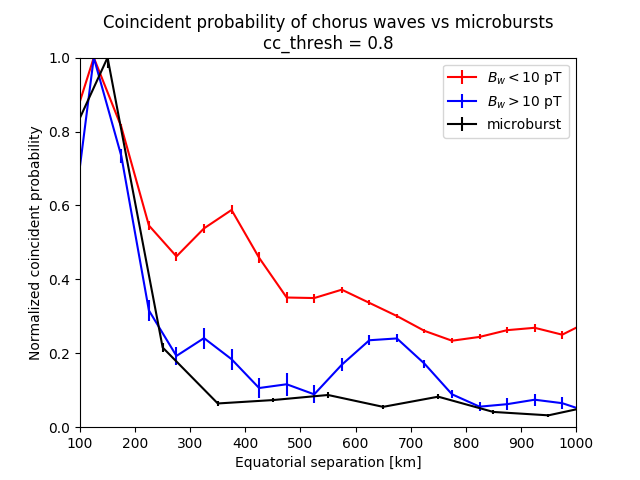
\includegraphics[width=\textwidth]{4_compare_chorus_microburst_fraction_cc_thresh_8.png}
\caption{Comparison of the highly correlated lower band whistler mode chorus wave distribution estimated by \citet{Agapitov2018} to the AC6 equatorial microburst distribution. The chorus waves were split up by wave amplitude into a low ($B_w < 10$ pT) and high amplitude ($B_w > 10$ pT) subsets. The red and blue curves show the probability of observing low or high amplitude, highly correlated chorus waves in each THEMIS separation bin. The black curve shows the AC6 equatorial microburst distribution in the same format. The errors bars show the standard error estimated using Poisson statistics.}
\label{fig_appendixc_1}
\end{figure}
